\documentclass[conference]{IEEEtran}

\usepackage[british]{babel}
\usepackage{cite}
\usepackage{graphicx}
\usepackage[hyphens]{url}
\usepackage{amsthm}
\theoremstyle{definition}
\newtheorem{definition}{Definition}
\usepackage[textstyle,squaren]{SIunits}
\usepackage[pdftex,colorlinks=true]{hyperref}


% correct bad hyphenation here
%\hyphenation{op-tical net-works semi-conduc-tor}


\begin{document}
%
% paper title
% can use linebreaks \\ within to get better formatting as desired
\title{Exploring UK Crime Networks}

% author names and affiliations
% use a multiple column layout for up to three different
% affiliations
\author{\IEEEauthorblockN{Giles Oatley}
\IEEEauthorblockA{Department of Computing\\
Cardiff Metropolitan University\\
Cardiff, UK\\
Email: goatley@cardiffmet.ac.uk}
\and
\IEEEauthorblockN{Tom Crick}
\IEEEauthorblockA{Department of Computing\\
Cardiff Metropolitan University\\
Cardiff, UK\\
Email: tcrick@cardiffmet.ac.uk}}

% conference papers do not typically use \thanks and this command
% is locked out in conference mode. If really needed, such as for
% the acknowledgment of grants, issue a \IEEEoverridecommandlockouts
% after \documentclass


% use for special paper notices
%\IEEEspecialpapernotice{(Invited Paper)}


% make the title area
\maketitle


\begin{abstract}
This paper describes our experiences with three different crime
networks in the UK: burglary, `gun' gangs and retail theft. We present
an introduction into each of these problems, and highlight some of the
issues related to over-simplification of the network analysis.

We also review the term `third-generation' analysis, and provide some
insights into achieving this, but also conclude that it can be an
extremely expensive (computational) undertaking.
\end{abstract}

% For peer review papers, you can put extra information on the cover
% page as needed:
% \ifCLASSOPTIONpeerreview
% \begin{center} \bfseries EDICS Category: 3-BBND \end{center}
% \fi
%
% For peerreview papers, this IEEEtran command inserts a page break and
% creates the second title. It will be ignored for other modes.
\IEEEpeerreviewmaketitle


\section{Introduction}\label{sec:introduction}
Social network analysis has been applied across a wide range of
domains, providing a unifying language to describe disparate systems
ranging from social interactions to power grids; there is also a
growing body of literature applied to crime analysis (see
\cite{Klerks2001,OatleyZeleznikowLearyEwart2005,OatleyEwartZeleznikow2006,BaronTindall1993,Hansen2005,CalvoArmengolZenou2006,PatacchiniZenou2008,HutchinsBenhamHutchins2009}).

Within the deterministic literature of criminology and crime
informatics we find what Klerks calls `third-generation'
analysis~\cite{Klerks2001}. The first generation (crime) analysis
techniques were the Anacpapa charts~\cite{harper+harris:1975} and maps
with coloured pins~\cite{OatleyEwart2003}. Second generation
techniques include the range of tools available to crime analysts,
from powerful freeware
(e.g. Pajek\footnote{\url{http://pajek.imfm.si/doku.php}}) to
mid-range solutions offering operationally useful measures beyond
standard social network analysis computations (e.g. IBM i2
COPLINK\footnote{\url{http://www.ibm.com/software/products/en/coplink/}}
and IBM i2 Analyst's
Notebook\footnote{\url{http://www.ibm.com/software/products/en/analysts-notebook/}},
ORA \cite{HutchinsBenhamHutchins2009}), to significantly more
expensive bespoke solutions (e.g. Detica
NetReveal\footnote{\url{http://www.deticanetreveal.com/}}). The second
generation techniques essentially provided graphical representations
of simple raw data. Actual content, let alone meaning of such contacts
was analysed only in a very crude way:

\begin{quote}
``{\emph{Social network analysis of the sort we could call `third-generation'
would focus much more intensely on the content of the contacts, on the
social context, and on the interpretation of such
information.}}''~\cite{Klerks2001}
\end{quote}
 
A number of
researchers~\cite{CalvoArmengolVerdierZenou2007,PatacchiniZenou2008}
offer a related approach, analysing the strength of weak ties in crime
through steady state equilibria modelling, however
Klerks~\cite{Klerks2001} was interested in understanding in a
qualitative way the behaviour, motivations and choices of the
individuals concerned and contributing to a better understanding of
vital social processes, power and affinity structures. Certainly there
are misconceptions within law enforcement. For instance:

\begin{quote} 
``{\emph{...many law enforcement practitioners...appear to
hold rather simplistic views of their adversaries: they often think in
rigid terms of leaders, chains of command, bag carriers and stable
criminal infrastructures where I observe mostly improvisation, fluid
networks and ad hoc coalitions, opportunistic and very flexible
individual entrepreneurs, criminal omnivores and organisational
chaos.}}''
\end{quote}

\noindent Furthermore: 

\begin{quote}
``{\emph{In short, social ties much more than business relations of formal
command structures form the basis for criminal
co-operation. Pyramid-like criminal authority structures are
increasingly rare, although within smaller cells such as nuclear
families the more traditional father-son-like authority relations can
still be found. (Semi-)independent criminal operators often work in
pairs of two, teaming up with several different co-operations instead
of belonging to one group.}}''
\end{quote}


\section{Disambiguating networks: the meaning of links}\label{sec:disambiguating}
Work with the crime type of burglary, in collaboration with West
Midlands Police in the UK, investigated the combination of social
network measures with spatial data. Links in this dataset were based
on codefendence. Incorporated directly into the \emph{betweenness}
calculation were values for offender range (geographical difference
between linked offenders), the `danger' of an offender (amount of
crimes committed) and the strength of links (product of amount of
co-crimes and recency of last crime)~\cite{OatleyEwart2005}.This
resulted in a weighted betweenness value that better reflected the
importance of an offender.

\begin{figure}[!ht] 
\centering
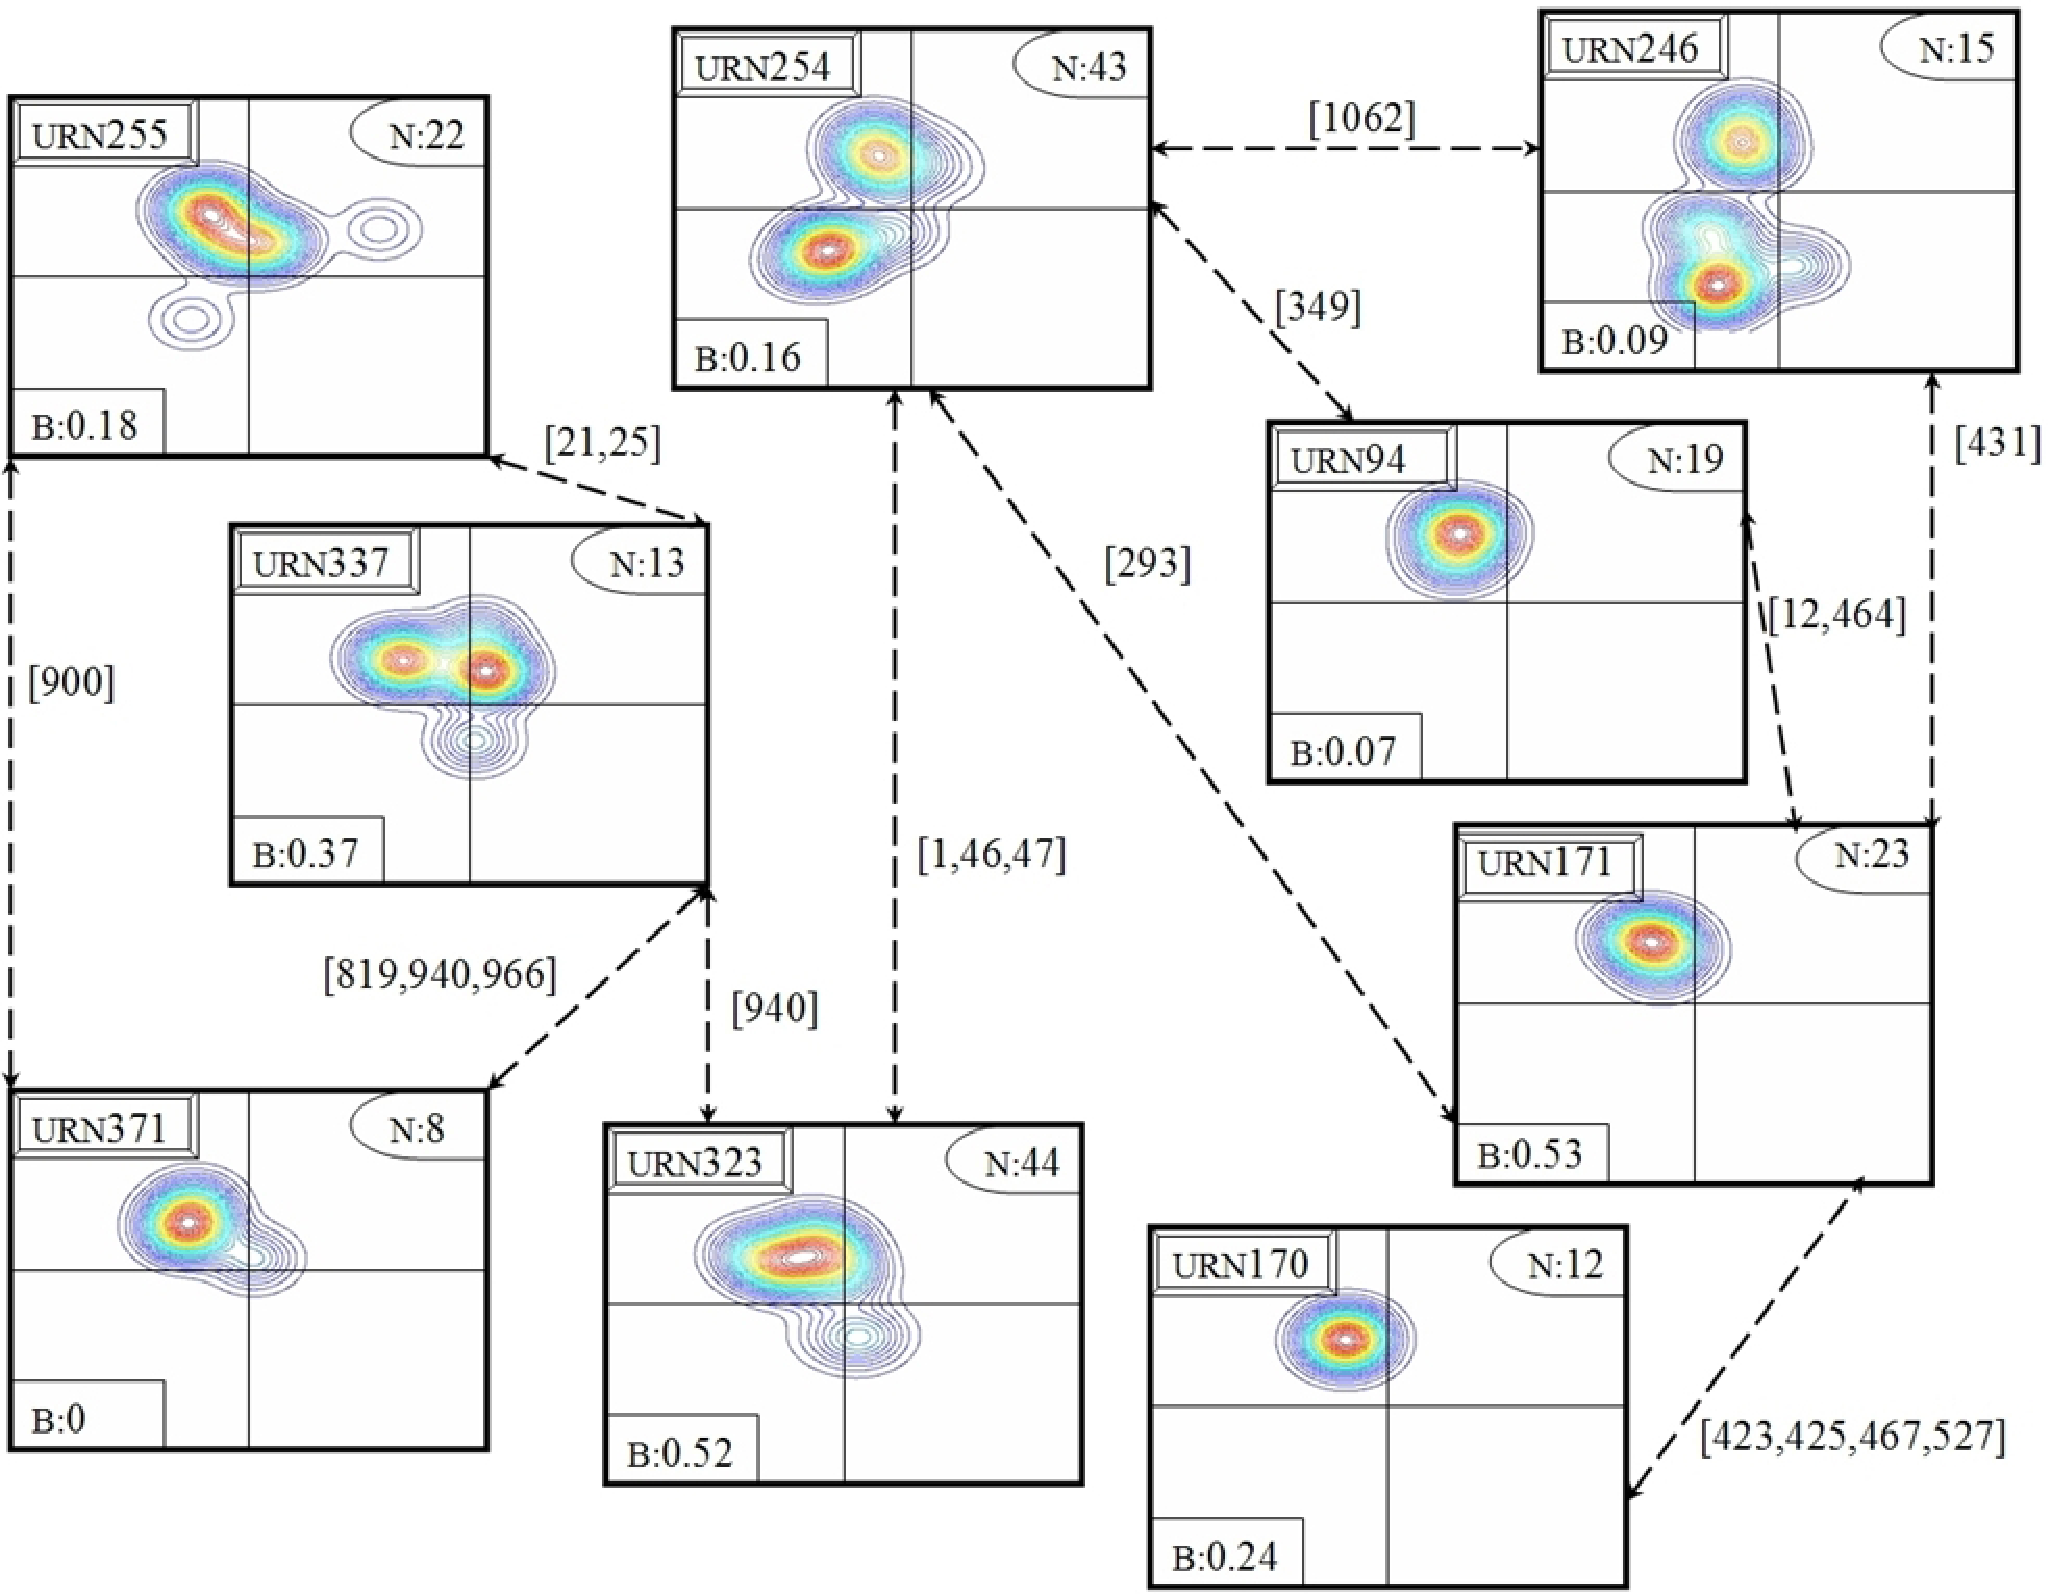
\includegraphics[width=\columnwidth]{images/burglary}
\caption{Geographical networks of burglars. Each of the 2x2 squares represents an offender, with Unique Reference Number (\emph{URN}), number of crimes (\emph{N}) and betweeness value (\emph{B}). The crime positions are displayed in interpolated form. The links between offenders are labelled with dates, as days from the start of the project. For instance Offenders 171 and 170 committed 23 and 12 crimes respectively, all roughly in the same geographical region, with four crimes together within a period of 104 (527-423) days. }
\label{fig:burglary}
\end{figure}

From the large networks of linked offenders (\emph{n}=17000), however
it was not clear whether the link could be considered strong or weak,
recent or old, and offender pairs committing many crimes together in
the recent past would appear the same as those offenders whose
activity together was a long time passed through only a single crime.

While the betweenness metric can be useful, it is clear that in the
case of crime types such as burglary there is also the need to consider
the spatial aspect. Consideration of the temporal and frequency
analysis of the crimes constituting the links will also provide a
better understanding of the nature of the links, and may highlight
links that are not considered significant by the betweenness metric.


\section{Gun gangs}\label{sec:manchester}
The UK has been slow in carrying out research into gang crime,
excepting Pitts~\cite{pitts:2007}, and especially into what actions
work best at controlling it. In Greater Manchester, a region in the
north of the UK that has had a significant gun crime
problem~\cite{BBCNews2003,BBCNews2004,HalesLewisSilverstone2006}
related to gang activity (primarily due to acute social deprivation in
the area), recent police initiatives have started to address this
problem~\cite{BBCNews2010}.

Reported elsewhere~\footnote{Submitted to ASONAM 2014, currently under
review.}, in collaboration with the UK's Greater Manchester Police, we
examined the dynamics of a social network study of these gangs and
their associates, using the intelligence gathered by police
observations of known gang members and associated criminals. Links
between offenders are a range of intelligence types, from codefendent
to `seen together'. This reinforces the value of using social network
analysis for gang research: identifying structural holes, betweenness
and social capital~\cite{papachristos:2006}.

Figure~\ref{fig:2000ganglabels} shows links between two rival gangs.  In
2000, Gangs A and B were rivals. These later divided in 2001 into Gang
C (from A) and into Gang D (from B) in 2004 -- see Figure~\ref{fig:all}. We
investigated this process based on local features (modularity,
cliques) and global features (clustering coefficient). Identifying the
changes in these could help us identify the possible birth of new
gangs (sub-networks) in the social system.

\begin{figure}[!ht] 
\centering
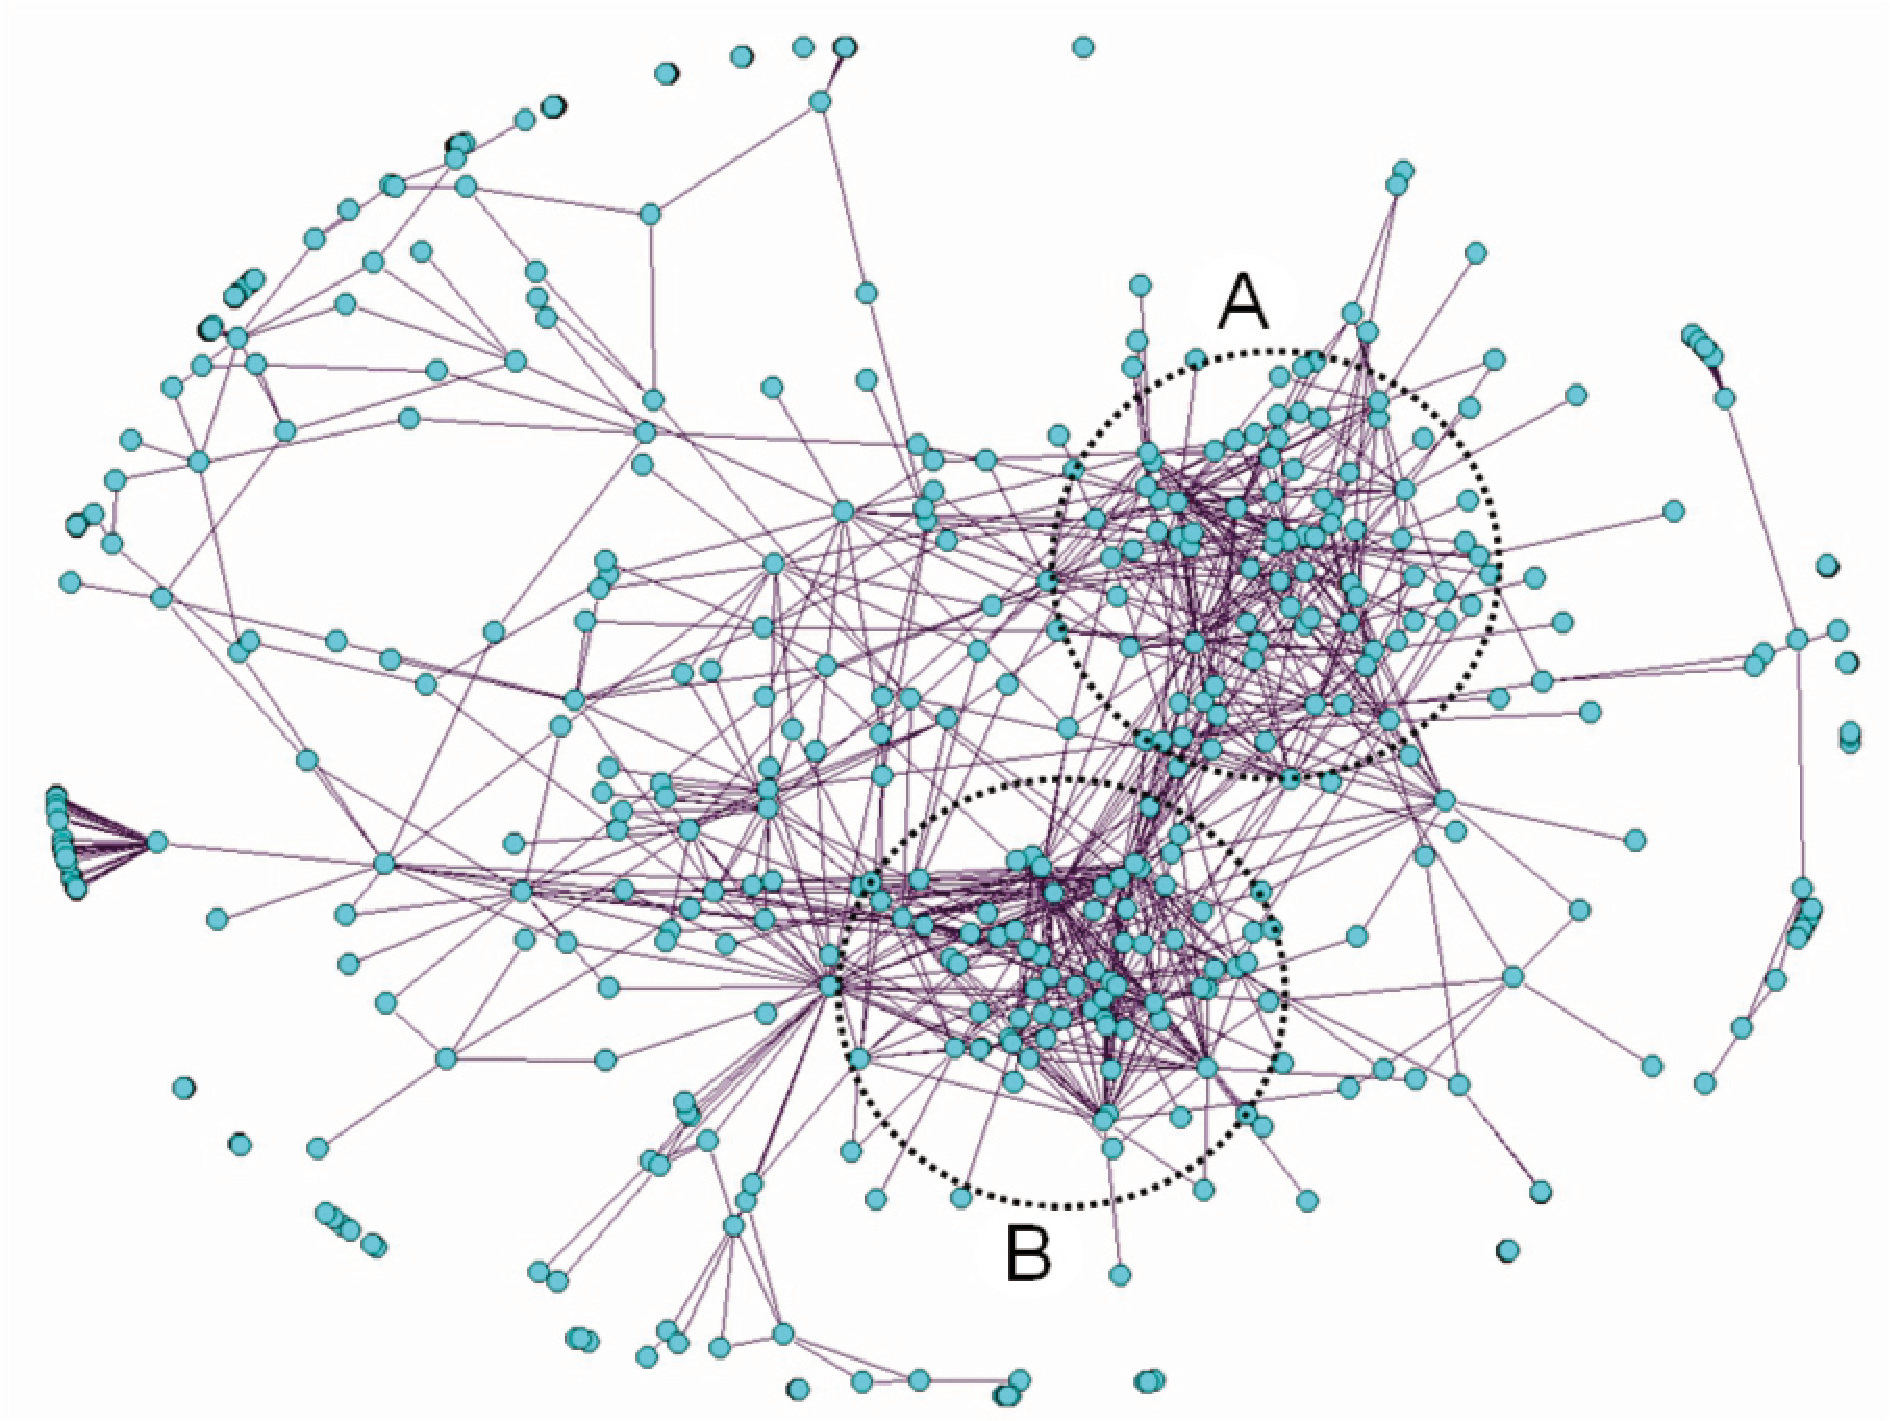
\includegraphics[width=\columnwidth]{images/2000ganglabels}
\caption{Rival gangs A and B.}
\label{fig:2000ganglabels}
\end{figure}

Studying the dynamics of these networks globally and locally, we
identified the global characteristics that tell us that they are not
random graphs -- they are small world graphs and therefore the
formation of gangs is not a random event. However, there is much more
to analyse, based on the specific nature of the links, and the complex
histories of each offender.

\begin{figure*}[!ht] 
\centering
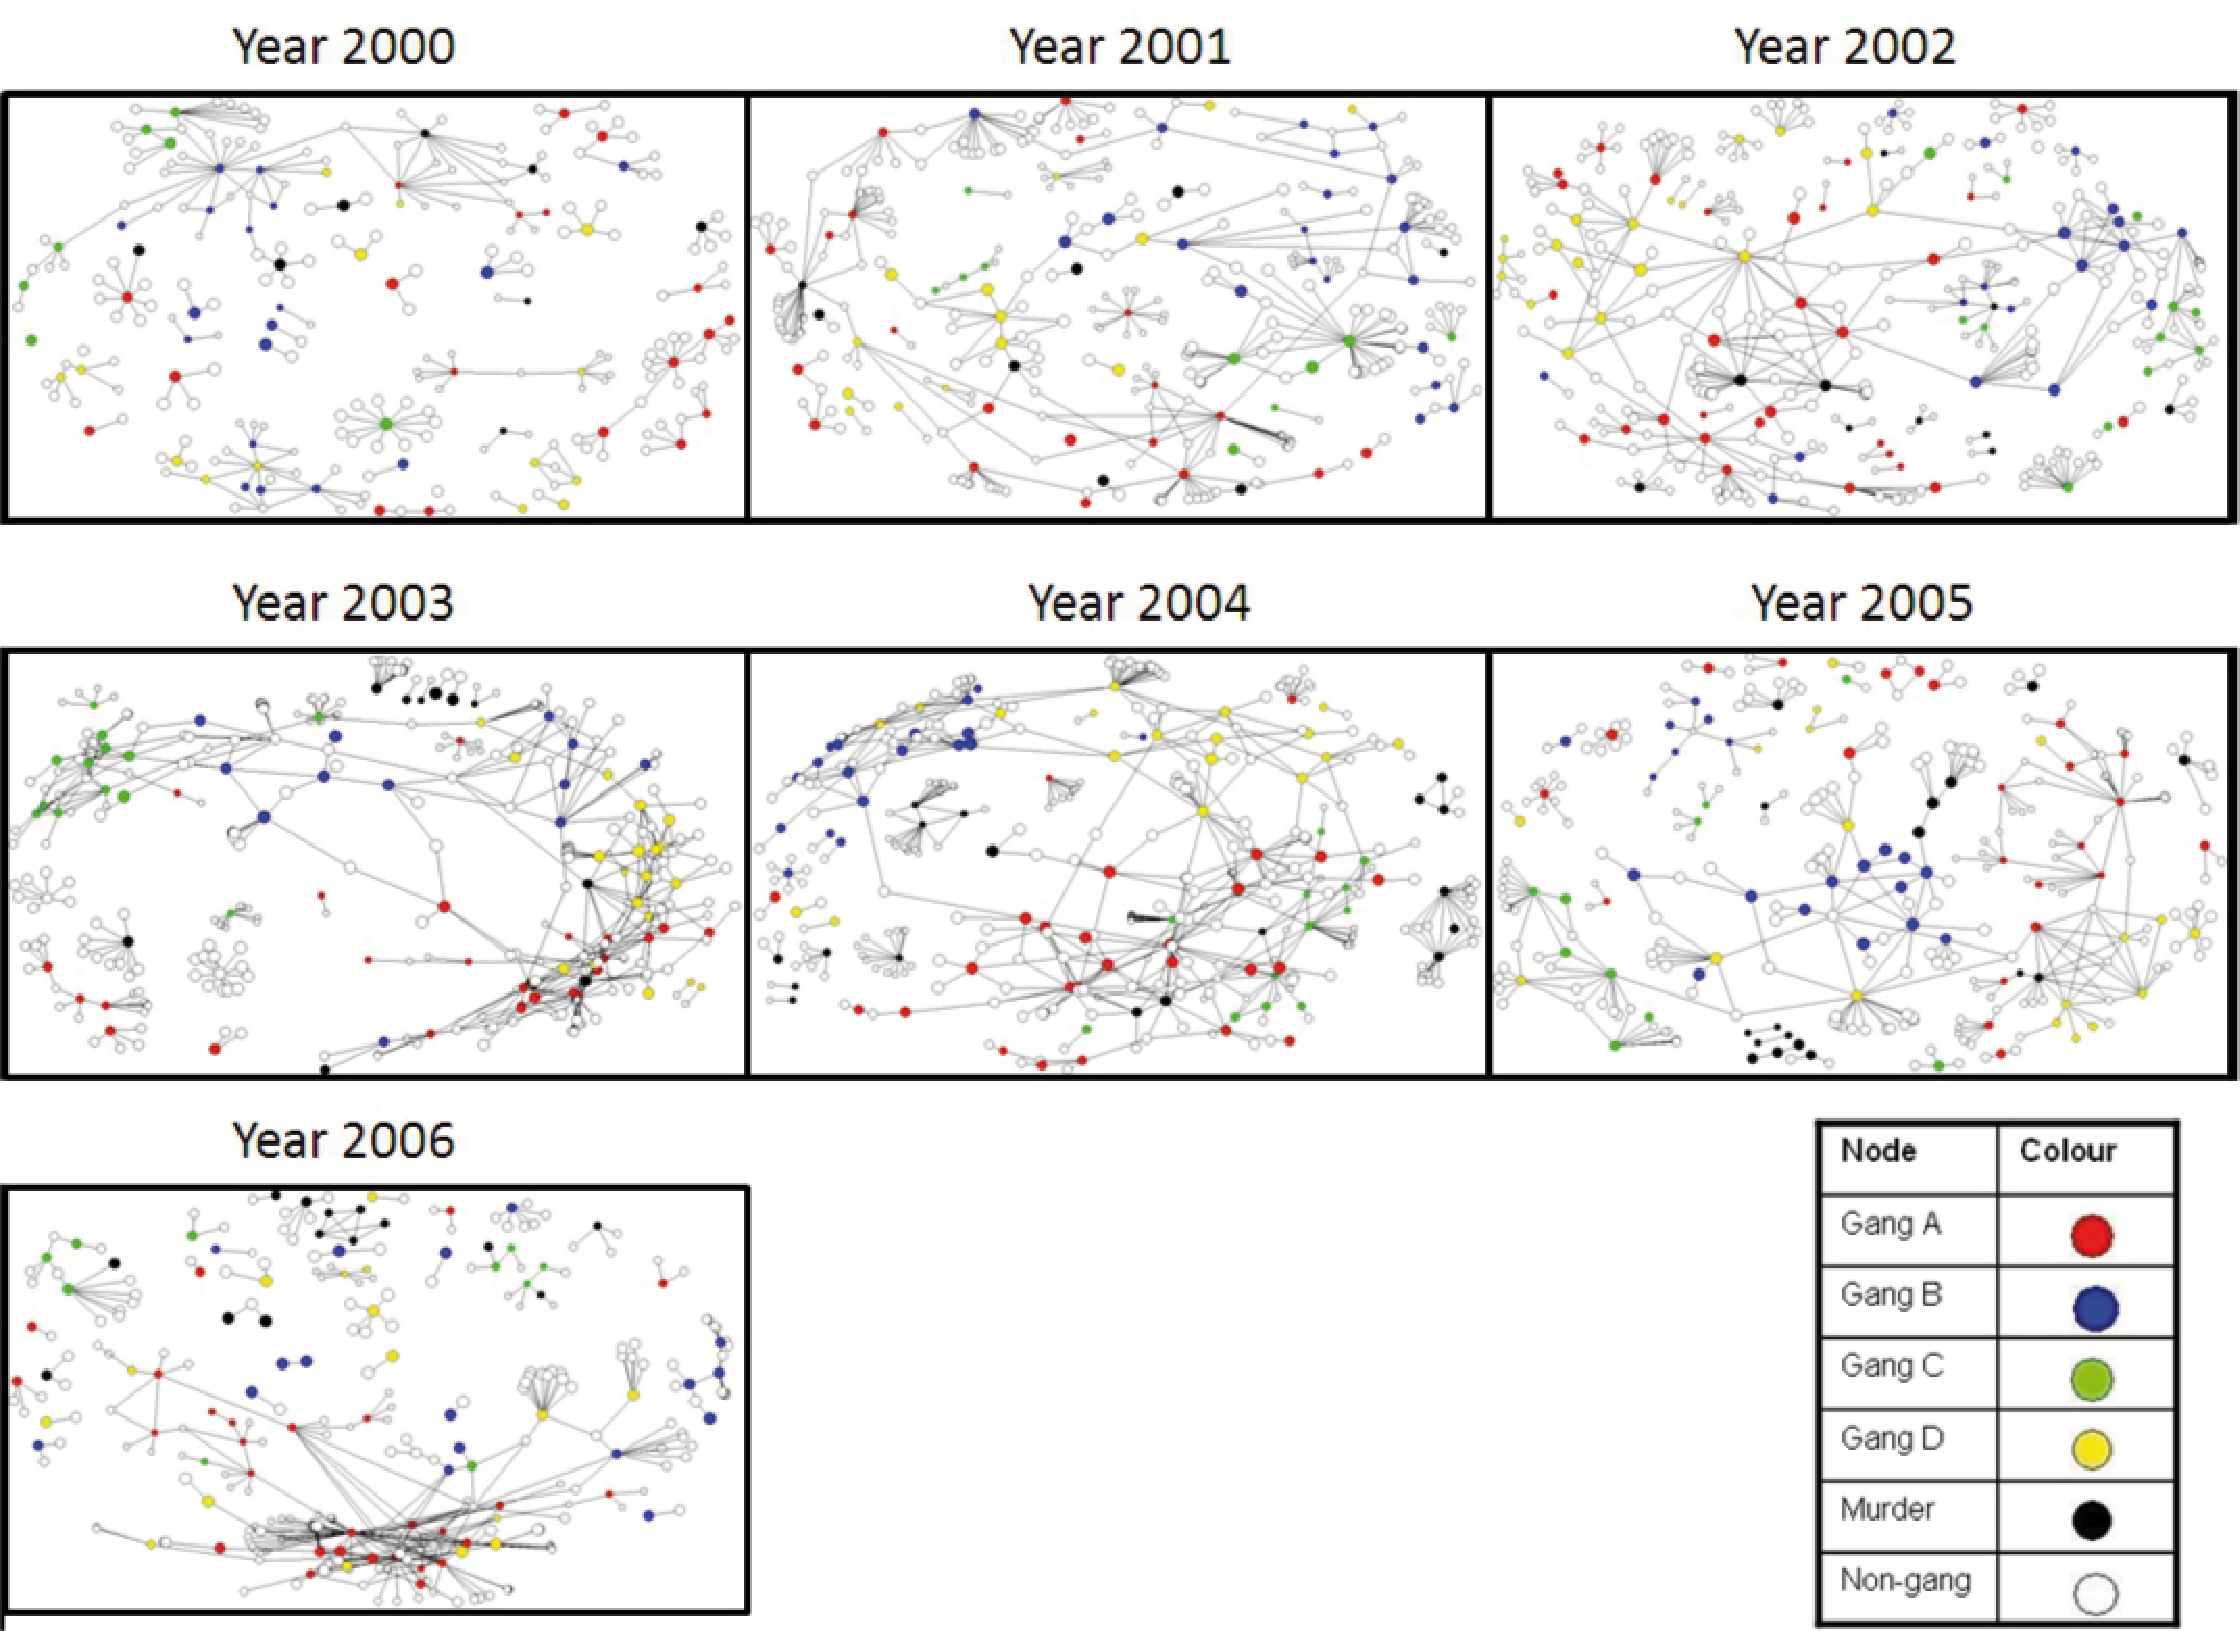
\includegraphics[width=\textwidth]{all}
\caption{Growth of networks. Showing the formation of annual links. Only nodes directly connected to a gang member are included.}
\label{fig:all}
\end{figure*}


\section{Third-generation analysis}\label{sec:thirdanalysis}
Recalling the definition presented earlier, `third-generation' social
network analysis focuses much more intensely on the content of the
contacts, on the social context, and on the interpretation of such
information. We are particularly interested in what constitutes the
bonding mechanisms that tie people together in different
constellations: greed, ethnic or tribal ties, family relations, common
geographical (neighbourhood) or institutional
(prison)~\cite{Klerks2001}.


\subsection{Specific gang roles}\label{sec:shortestpaths}
% is this the right Aldridge ref??
There are many definitions of gangs; for instance
Pitts~\cite{pitts:2007} reviews a plethora of definitions and
typologies, eventually developing their own six-point typology for
their particular study.  Aldridge et al.~\cite{aldridge-et-al:2008}
recognise the messiness and looseness of the social networks referred
to as gangs, as well as their permeable and fluctuating boundaries.
In contrast, Pitts~\cite{pitts:2008} claims, arguably without
providing much evidence for it, that we are witnessing the development
of new articulated `supergangs' with long histories of involvement in
organised crime, clear subgroups, role differentiation, established
territories and neighbourhood control, vertical links into higher
echelon organised crime, and organised drug dealing activity.

The \emph{degree} values from our analysis the the gangs suggested
that there are no obvious single leaders, however intelligence
suggests that South Manchester gangs in the UK do appear to have a
basic system of hierarchy. Gang's A and B members store firearms at
the home addresses of younger affiliates of the gang, who are eager to
prove themselves to `superior' members of the gang. The roles within
the gangs include the following:

\begin{itemize}
\item \emph{Leader:} responsible for recruiting new members.
Sanctions the enforcers to carry out `missions' on their behalf and
authorises who carries the firearm.
\item \emph{Provider:} an individual either internal or external to
the gang able to supply firearms and/or ammunition.
\item \emph{Enforcers/riders:} nominated individuals who are active
gunmen for the gang. `Riders' are used as support to the gunmen with
three or four riders to one gunman.  They surround the gunmen on bikes
until the target is in sight, also acting as decoys should the group
attract police attention. They ensure that the gunman will get away
whilst they are stopped and questioned.
\item \emph{Runners/dealers:} members of the gang who distribute and
supply drugs, usually on the leaders behalf, usually the younger
element of the group.
\end{itemize}
  
It is important to note that these defined roles give the impression
of organisation within the group however the lifestyle of gang members
is often disorganised and unplanned. Detailed qualitative/ethnographic
descriptions tend to portray gangs as loosely-structured groups that
lack clear role expectations and stable
leadership~\cite{hughes:2005}. Firearms incidents between gangs are
sporadic in their nature and often have the hallmarks of chance
encounters with members of opposing gangs, which makes them difficult
to anticipate.

We should also be careful when looking at data and creating networks
from it. However, Klerks~\cite{Klerks2001} cites the case of the
`conspiracies' and mega-hierarchies that police had identified in the
past among Dutch and Turkish organised crime which were in fact
strings of interlinked smaller groups that lacked a central leader but
that coordinated their activities along logistic trails and through
bonds of friendship.


\subsection{Link analysis}
We require a better analysis of link types, for instance in the study
by Patacchini and Zenou~\cite{PatacchiniZenou2008} of whether weak
ties play an important role in explaining criminal activities. They
developed a model where individuals learn about crime opportunities by
interacting with other peers. The theoretical predictions of the model
are confirmed by the empirical analysis since they find that weak
ties, as measured by friends of friends, have a positive impact on
criminal activities.

To give a better idea of the interconnectedness of the gangs, the
following Figures~\ref{fig:chain2001} and \ref{fig:chain2004}) demonstrate
\emph{cycles} in the data, passing from one gang to another via
intermediaries.  These examples have been chosen from the 2001 and
2004 data when the new gangs emerged. Plotted in this way we can see
the complex relationships between (rival and sympathetic) offenders in
this geographically small region.

Furthermore, for 2001 and 2004, it would be interesting to examine the
kinds of links within each gang which emerged.

\begin{figure}[!ht] 
\centering
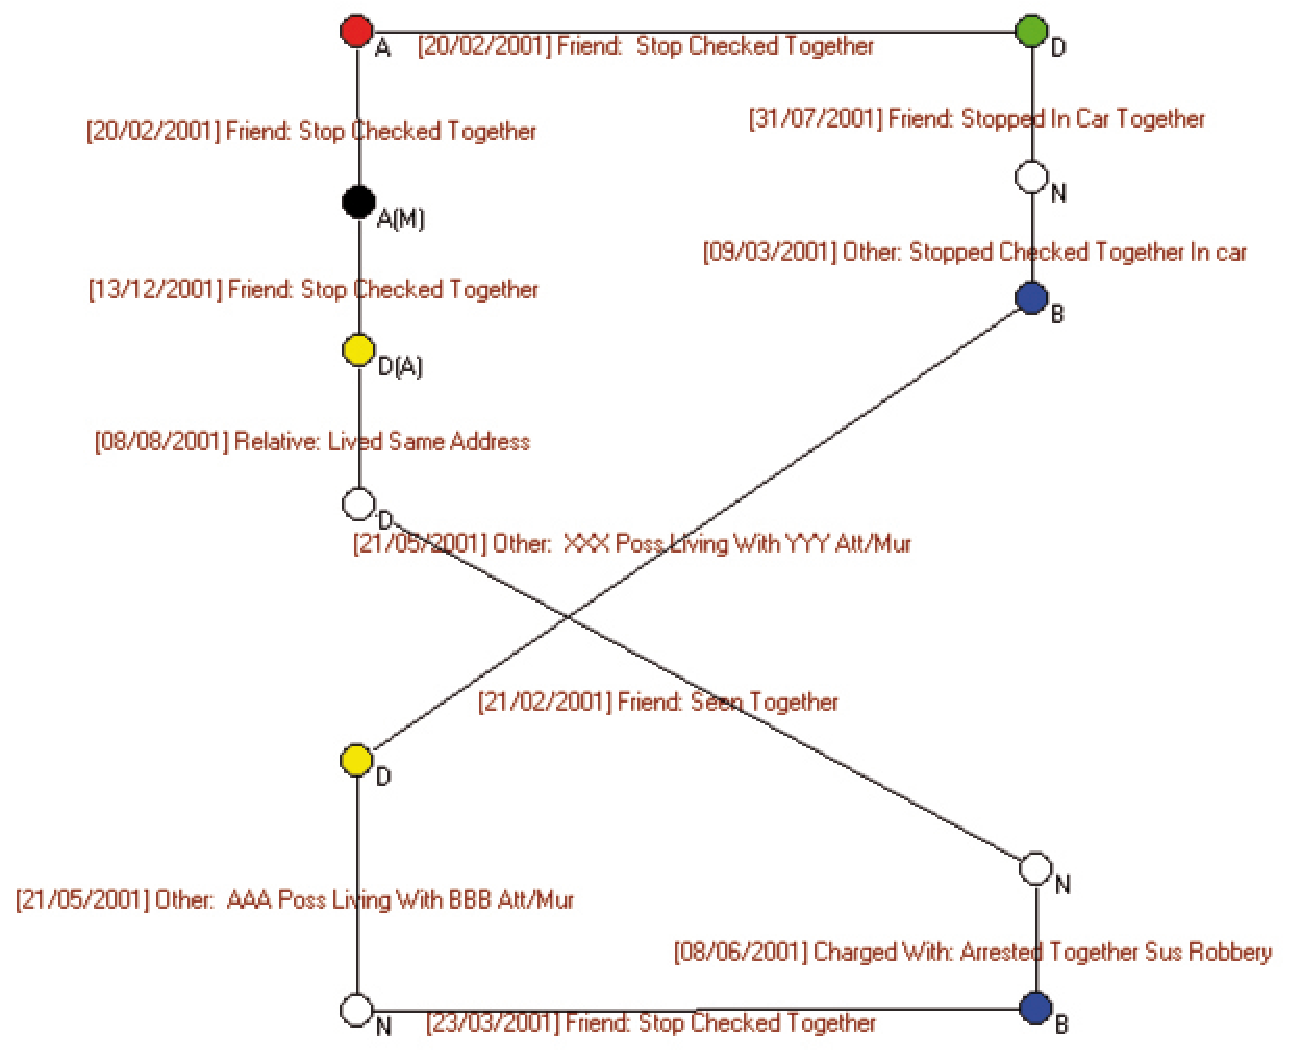
\includegraphics[width=\columnwidth]{images/chain2001}
\caption{Cycle (2001). The tension is between Gangs A (red), B (blue),
 C (green) and D (yellow). A(M) is a member of the Gooch gang (Gang A), however they are coloured black to represent the crime of murder.}
\label{fig:chain2001}
\end{figure}


\begin{figure}[!ht] 
\centering
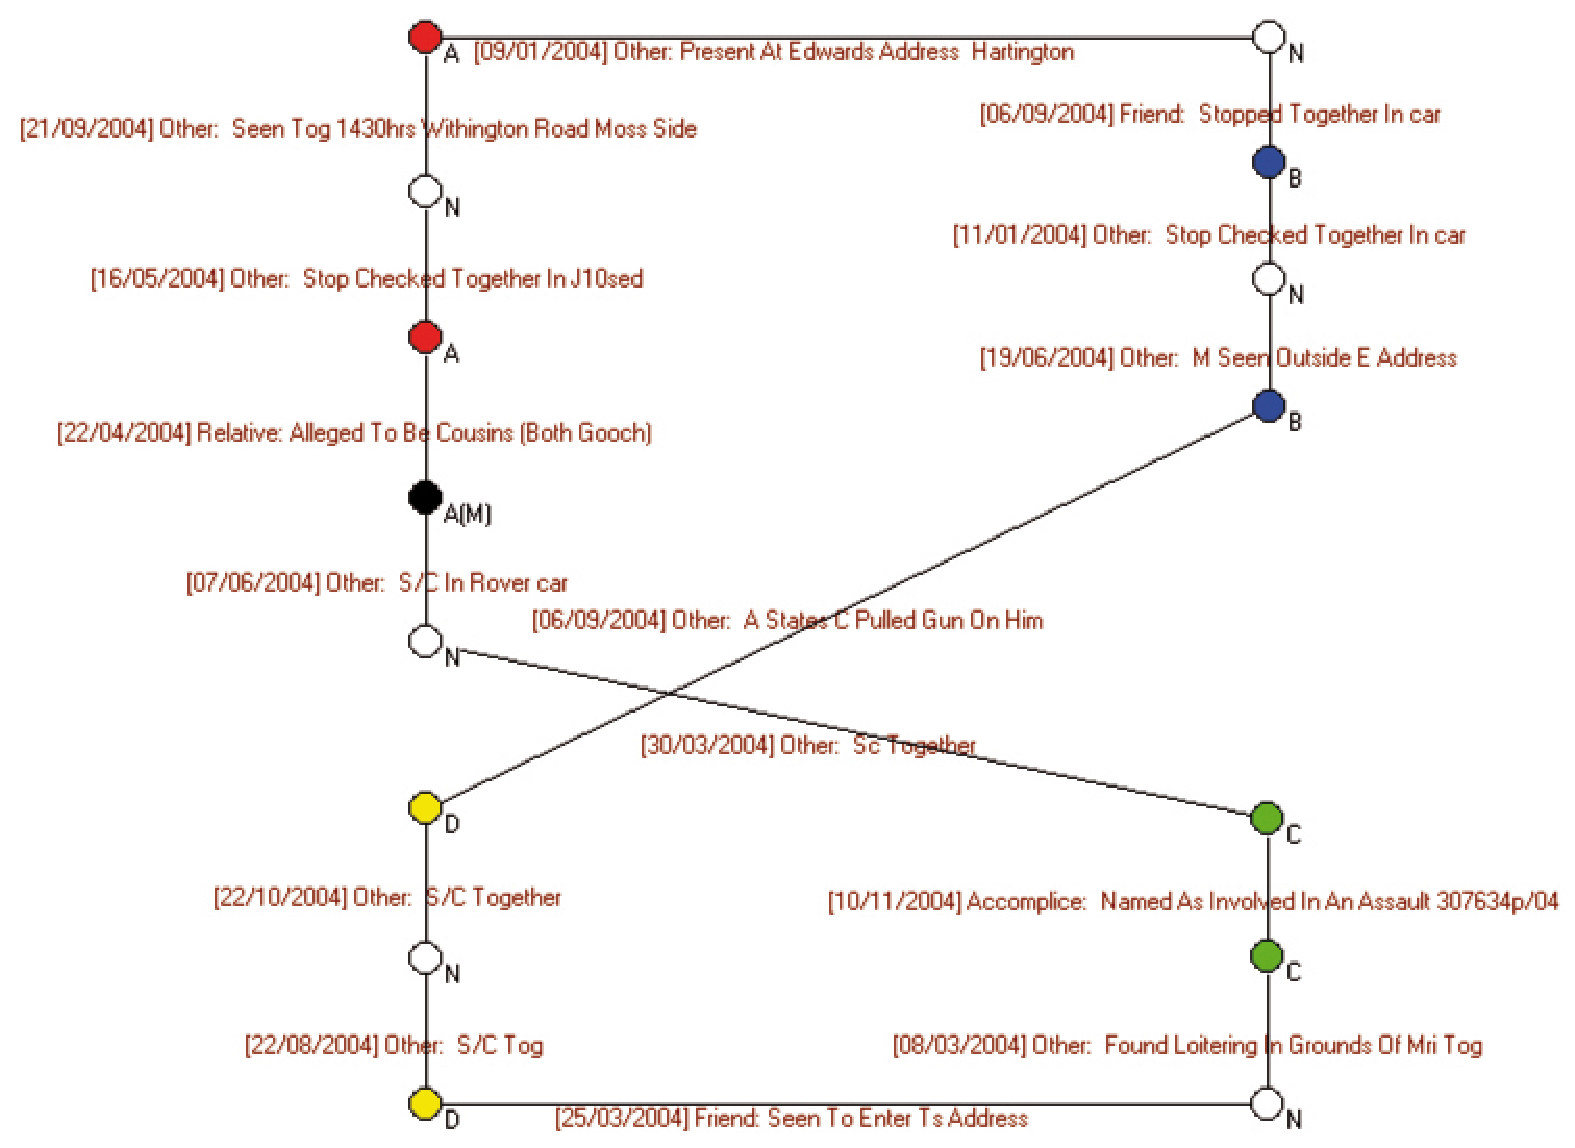
\includegraphics[width=\columnwidth]{images/chain2004}
\caption{2004 cycle; the tension is between Gangs A (red), D (yellow) and B (blue), C (green).}
\label{fig:chain2004}
\end{figure}

\subsection{Node analysis}
Table~\ref{tab:histories} shows the sequence of accused crimes for
three members of the Gooch gang. Column one shows the first gang
member with a `profile' strongly related to robbery, in contrast to
the second and third gang members with `profiles' involving gun crime
and serious crimes. It is clear from studying these data that not all
gang members are gun users.


\begin{table*}[!ht]
  \centering
\resizebox{\textwidth}{!}{
    \begin{tabular}{lll}
    %%\addlinespace
    %%\toprule
    \textbf{Gooch 1} & \textbf{Gooch} 2 & \textbf{Gooch 3} \\
    %%\midrule
    ROBBERY - PERSONAL      & ROBBERY               & DAMAGE OTHER           \\
    S.5 PUBLIC ORDER ACT    & ROBBERY               & OFFENSIVE WEAPON       \\
    THEFT/TAKE PEDAL CYCLE  & ASSAULT S. 47         & ROBBERY - BUSINESS     \\
    THEFT OF MOTOR VEHICLE  & THEFT FROM THE PERSON & POSSESS CANNABIS       \\
    GOING EQUIPPED          & ASSAULT S. 47         & TAKING A MOTOR VEHICLE \\
    ROBBERY - BUSINESS      & ASSAULT S.18          & ARSON                  \\
    THEFT OF MOTOR VEHICLE  & RACIAL COMMON ASSAULT & BURGLARY DWELL OTHER   \\
    MAKE OFF W/O PAYMENT    & DAMAGE OTHER          & ATTEMPTED MURDER       \\
    ROBBERY - BUSINESS      & POSSESS HEROIN        & ATTEMPTED MURDER       \\
    ROBBERY - PERSONAL      & THEFT IN DWELLING     & ATTEMPTED MURDER       \\
    BREACH: ANTI-SOC. ORDER & ASSAULT S. 47         & ROBBERY - PERSONAL     \\
    THEFT FROM MV           & POSSESS UNSPEC. DRUG  & ROBBERY - PERSONAL     \\
    VIOLENT DISORDER        & COMMON ASSAULT        & ATTEMPTED MURDER       \\
    ROBBERY - PERSONAL   & ASSAULT S. 47           & POSSESS FIREARM ETC.    \\
    BURGLARY OTD OTHER   & WITNESS INTIMIDATION    & FIREARMS ACT OFFENCES   \\
    ROBBERY - BUSINESS   & ASSAULT S. 47           & ATTEMPTED MURDER        \\
    ROBBERY - BUSINESS   & ASSAULT S. 47           & ATTEMPTED MURDER        \\
    ROBBERY - BUSINESS   & RECEIVING STOLEN GOODS  & POSSESS FIREARM ETC.    \\
    ROBBERY - BUSINESS   & S.5 PUBLIC ORDER ACT    & FIREARMS ACT OFFENCES   \\
    ROBBERY - BUSINESS   & DAMAGE (MOTOR VEHICLE)  & POSSESS CANNABIS        \\
    ROBBERY - BUSINESS   & ASSAULT S. 47           & POSSESS FIREARM ETC.    \\
    ROBBERY - BUSINESS   & BREACH: ANTI-SOC. ORDER & FIREARMS ACT OFFENCES   \\
    ROBBERY - BUSINESS   & MURDER (OVER 1 YEAR)    & FIREARMS ACT OFFENCES   \\
    BURGLARY DWELL OTHER & POSSESS CANNABIS        & RAPE OF FEMALE UNDER 16 \\
    ROBBERY - BUSINESS   & POSSESS CANNABIS W/I    & ROBBERY - PERSONAL      \\
    ROBBERY - PERSONAL   & ASSAULT S.18            & ATTEMPTED MURDER        \\
    ROBBERY - BUSINESS   & ASSAULT S.18            & DANGEROUS DRIVING      \\
    ROBBERY - BUSINESS   & BREACH: ANTI-SOC. ORDER & SUPPLY/OFFER CANNABIS  \\
    ROBBERY - BUSINESS   & BREACH: ANTI-SOC. ORDER & POSSESS CANNABIS       \\
    MAKE OFF W/O PAYMENT & ROBBERY - PERSONAL      & POSSESS CLASS A W/I    \\
    ROBBERY - BUSINESS   & BREACH: ANTI-SOC. ORDER & KIDNAPPING             \\
    BURGLARY OTD         & BREACH: ANTI-SOC. ORDER & THEFT OF MOTOR VEHICLE \\
    ROBBERY - BUSINESS   &       & POSSESS CANNABIS       \\
    ROBBERY - BUSINESS   &       & ASSAULT POLICE         \\
    ROBBERY - BUSINESS   &       & ASSAULT POLICE         \\
    ROBBERY - BUSINESS   &       & ASSAULT POLICE         \\
    ROBBERY - BUSINESS   &       & POSSESS CANNABIS       \\
    ROBBERY - BUSINESS   &       & THEFT OF MOTOR VEHICLE \\
    ROBBERY - PERSONAL   &       & MANSLAUGHTER           \\
          &       & POSSESS CANNABIS       \\
          &       & S.5 PUBLIC ORDER ACT   \\
          &       & ABSCOND LAWFUL CUSTODY \\
          &       & BURGLARY OTD OTHER     \\
          &       & KIDNAPPING             \\
          &       & ROBBERY - PERSONAL     \\
          &       & ROBBERY - BUSINESS     \\
          &       & MURDER (OVER 1 YEAR)   \\
          &       & MURDER (OVER 1 YEAR)   \\
    %%\bottomrule
    \end{tabular}}
 \caption{Example offender histories in chronological order; all three offenders belong to
   the Gooch gang (Gang A).}
  \label{tab:histories}
\end{table*}


\section{Retail Offending Teams}\label{sec:retail}
Retail is one of the largest economic sectors in the UK, yet the
impact of criminal activity in this domain has received relatively
little attention.  Customer theft of goods from shops can account for
almost half of stock loss, but there have been few studies on this
issue. There is an clear need for more research and Ewart and
Tate~\cite{EwartTate2007} discuss how the investigation of retail
offending is able to draw upon a body of criminological findings and
methodologies~\cite{Bamfield2006}.

A unique database was used, held by the UK's North East Retail Crime
Partnership (NERCP)~\footnote{\url{http://www.nercp.org.uk/}}.  This
is a partnership between 29 retail chains, 11 shopping centres, 6
town/city centre partnerships and 4 police forces in the North East of
England.  It has extensive data sharing links to other regional
partnerships across the UK.  This includes Yorkshire and Humber
Business Crime Forum and the Scottish Business Crime Centre and a
further 11 police forces feed into the system. Information on over
30,000 offenders and 102,000 incidents in any twelve month period are
recorded and include admitted cases reported to the police as well as
those where the retailer has chosen not to report. Despite an emerging
operational need, there are no studies of retail criminality, therfore
there is a need to explore the organised teams of offenders.

\subsection{Motivation for the study}
The proportion of shop theft/refund abuse committed with the objective
of determining an empirical basis for informing targeting
priorities. The problems of aggregated data~\cite{TownsleyPease2002}
are addressed by using a disaggregated approach to establish more
precisely the geographical nature of `prolificness'. We expect a
team’s activities to be more geographically dispersed in comparison to
members' individual offending.

The constitution, stability and roles within teams with the objective
of informing detection and prevention strategies.  We expect to
identify key individuals who provide the core and temporary members
who are brought in for specific purposes such as the distraction of
security staff. The offending patterns of commuting teams and explore
geographic/temporal factors associated with target selection with the
objective of informing detection and prevention strategies.  We expect
to identify factors associated with target selection and delineate
teams according to offending patterns. 

\subsection{Retail theft data}
All NERCP data is collected using the National
Information/Intelligence Report Form
(5x5x5)~\footnote{\url{http://www.hmrc.gov.uk/manuals/mlr3cmanual/mlr3c14000.htm}}
approved by Association of Chief Police Officers (ACPO) and conforms
to standards required by Police National Intelligence
Model~\cite{john+maguire:2004}.

The data comprises information recorded by retailers on sightings of
known offenders and all incidents of shop theft and refund abuse
detected in their stores (whether subsequently reported to the police
or not) and includes biographical details of the offenders.  Detected
crimes are defined by the apprehension of the offender. The study is
anchored to the North East England in that the travelling patterns of
offenders based in this region are explored and contrasted with
information on those travelling too the region. Detections and
sightings are analysed to derive an empirical definition of `a team'
of offenders and explore a typology related to membership stability,
offending range or type of offending.

A preliminary analysis of NERCP data on one police force area reveals
that prolific offenders more often act in teams. Thirty people
committed between 17 and 44 offences of retail crime during 2006 and
24 of them committed almost all their offences with more than one
other.  All these `team players' have a large criminal range and
operate across two or more police force areas.
 
There are also no studies of retail criminality that explores
offenders who travel widely to commit their offences.  Findings from
burglary~\cite{Barker2000,EwartOatley2003,EwartOatley2006} suggest
locations will be significant to at least one of the group members, or
a retail chain may be targeted across the country because a corporate
strategy produces similar security systems in all its stores.  Little
is known of their offending patterns in a chosen area.  They may
`forage’~\cite{JohnsonBowers2004} where numerous premises within a
relatively small geographical range are targeted.  Alternatively, they
may `hit and run' a few shops over a wider area to avoid
detection. Understanding the temporal and geographical characteristics
of offending have provided important crime prevention and detection
information, yet retail offending remains to be explored in this way.


\subsection{Identifying teams of retail offenders}\label{sec:identifyteams}
Intelligence had identified nearly 20 gangs with identifiable modus
operandi and/or membership (e.g. family, or from a specific
geographical region). We were interested to see if we could find these
gangs by automatically partitioning the data. In this way, if we are
able to find our known gangs in certain partitions of the data,
perhaps un-labelled partitions might indicate previously unknown
gangs.

Our tangled network of relations consisted of 31106 vertices with
12742 edges. We used weak components method to partition the data,
with increasing number of nodes. The resulting partitions or list of
networks were extracted. Figure~\ref{fig:partitions} shows the log of
partitions against number of nodes. Actual values of nodes versus
partitions (for \emph{n}<=10) were: 1-22133, 2-3807, 3-926, 4-320,
5-153, 6-93, 7-67, 8-49, 9-34, 10-26. That is, when we considered
networks to be of size 1 node, then we found 22133 members or
partitions. When we considered networks to be of size 2 node, then we
found 3807 members or partitions, and so on. The size we initially
decided to investigate was 10-node weak components with a resultant of
26 partitions or sub-networks.


\begin{figure}[!ht] 
\centering
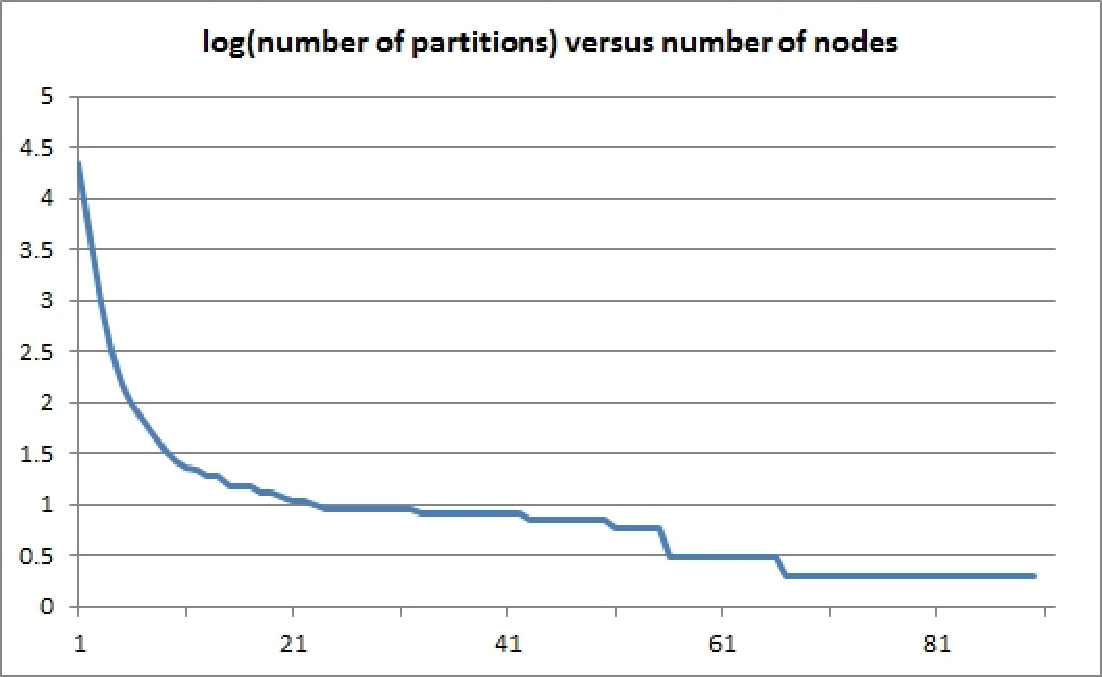
\includegraphics[width=\columnwidth]{images/partitions}
\caption{Number of nodes against number of partitions.}
\label{fig:partitions}
\end{figure}

Of the 20 known gangs we were able to identify 12 from our partitions,
or at least 12 networks that had at least one member from the gang
members. However it was initially surprising to see how interconnected
several of the gangs were. Using \emph{shortest paths} we identified
the following paths between the following gang's (anonymised to):
\emph{CM}, \emph{AR} and \emph{SEA}.


\begin{figure}[!ht] 
\centering
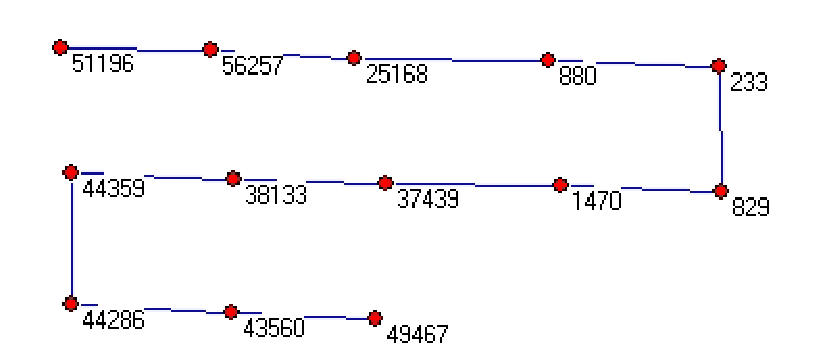
\includegraphics[width=\columnwidth]{images/path1}
\caption{Shortest path between Offender 49467 (Gang CM) and Offender 51187 (Gang AR).}
\label{fig:path1}
\end{figure}


\begin{figure}[!ht] 
\centering
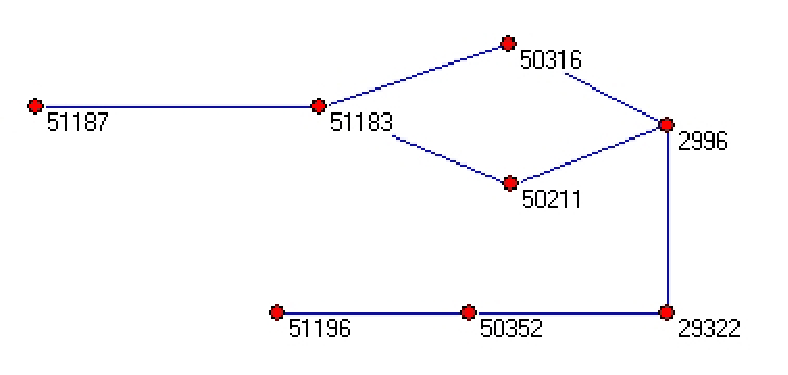
\includegraphics[width=\columnwidth]{images/path2}
\caption{Shortest path between Offender 51187 (Gang AR) and Offender 51196 (Gang SEA).}
\label{fig:path2}
\end{figure}


\begin{figure}[!ht] 
\centering
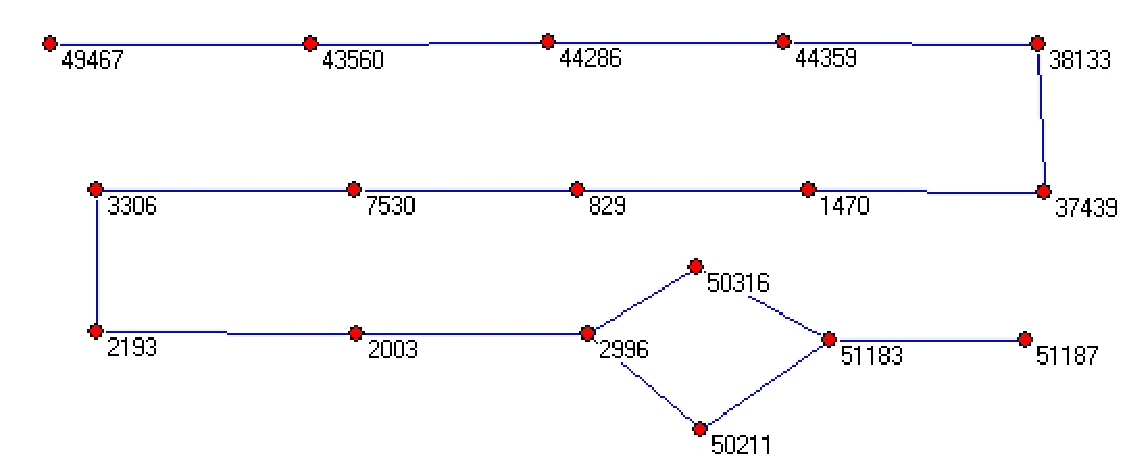
\includegraphics[width=\columnwidth]{images/path3}
\caption{Shortest path between Offender 51196 (Gang SEA) and Offender 49467 (Gang CM).}
\label{fig:path3}
\end{figure}


\section{Discussion}\label{sec:discussion}
The picture painted by the initial social network plot is quite
misleading in all three cases we have presented. The burglary data
required spatial data and other features to really start to understand
the meaning of the links between
offenders~\cite{JohnsonBowers2004,EwartOatley2005}. In the gun gangs,
the police held hypothesis of two rival sets of gangs is potentially a
misrepresentation of the much more complex sets of smaller cliques and
fluid changes within the larger gang structures. Not only are the
links between offenders of very different natures, but the nodes or
offenders themselves are very different as well. How to represent the
changing nature of an individual is something we have looked at
elsewhere. Finally then the very complex data of retail crime, with a
fraction of known gangs, presents its own particular challenges, of
how to make use of quite detailed intelligence on individuals (in
textual format) and combine with mining of the social networks.


\section*{Acknowledgments}
We acknowledge the contributions from the UK's Greater Manchester Police,
West Midlands Police and North East Retail Crime Partnership.

% trigger a \newpage just before the given reference
% number - used to balance the columns on the last page
% adjust value as needed - may need to be readjusted if
% the document is modified later
%\newpage
\IEEEtriggeratref{14}
% The "triggered" command can be changed if desired:
%\IEEEtriggercmd{\enlargethispage{-5in}}

% BibTeX users
\bibliographystyle{IEEEtran}      % basic style, author-year citations
\bibliography{fosint-si2014}   % name your BibTeX data base

\end{document}

